\begin{tcolorbox}[colback=blue!5!white,colframe=blue!75!black,title=Variador de velocidad]
	Es utilizado para controlar la velocidad de giro de un motor.
	Para regular las revoluciones, se debe tener en cuenta las características del motor, ya que este tiene una curva propia de funcionamiento. Un variador es capaz de generar elementos control de aceleración, frenado, seguridad, control del torque y operaciones que mejoran la eficiencia energética.
\end{tcolorbox}

\subsubsection{Especificaciones}
El variador de velocidad que se utilizó pertenece a la marca \textbf{Schneider Electric} (Figura \ref{fig:variador}) y posee las siguientes características.
\paragraph*{Altivar 312}
\begin{minipage}[t]{.5\textwidth}
	\begin{itemize}
		\item 	Modelo: ATV312HU15N4
		\item   Tensión: 380-500 V
		\item 	Frecuencia: 50/60 Hz
		\item 	Potencia: 1.5kW / 2 HP
		\item 	Fases: 3
	\end{itemize}
\end{minipage}
\begin{minipage}[t]{.5\textwidth}
	\centering\raisebox{\dimexpr \topskip-\height}{%
		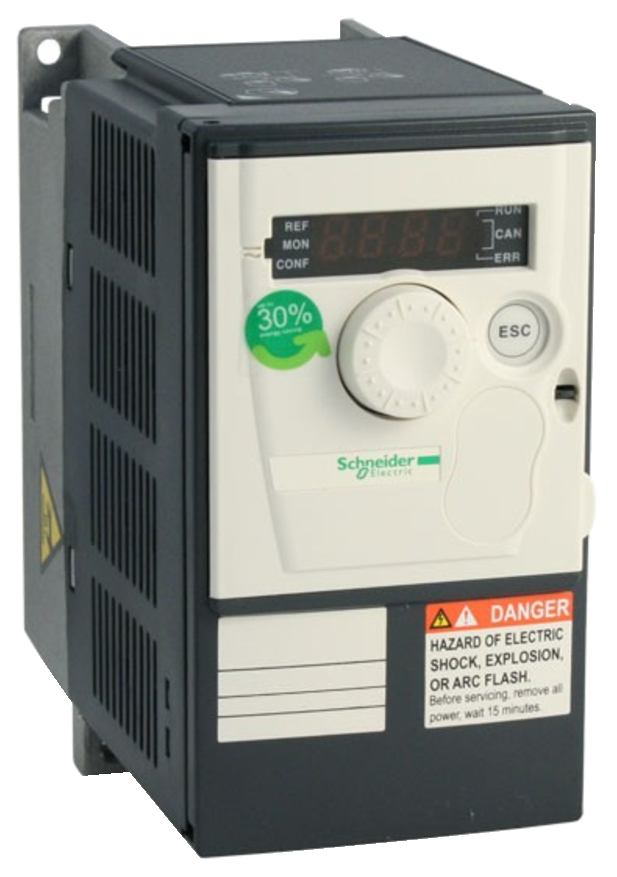
\includegraphics[scale=0.25]{variador.eps}}
	\captionof{figure}{Variador Altivar 312}
	\label{fig:variador}
\end{minipage}


Cabe destacar que el variador estima la velocidad de acuerdo a los parámetros del motor, por lo que para medir la velocidad verdadera se utiliza un \hl{FALTA ESTO, VA ACA O EN MOTOR??}


\subsubsection{Configuración de parámetros primarios}
Para realizar la configuración del motor se utilizó el software SoMove. Se descargó la ultima versión desde la página oficial de Schneider\footnote{\url{https://www.se.com/ar/es/product-range-presentation/2714-somove/}} y luego, la librería DTM correspondiente al variador a utilizar\footnote{\url{https://www.se.com/ar/es/download/document/Altivar_DTM_Library/}}.
\\
Una vez realizado esto se procedió a generar un nuevo proyecto eligiendo las características del variador (Figura \ref{fig:so2}). El próximo paso fue realizar por medio del software la carga de los parámetros del motor (Figura \ref{fig:so4}).
\begin{figure}[h]
	\centering
	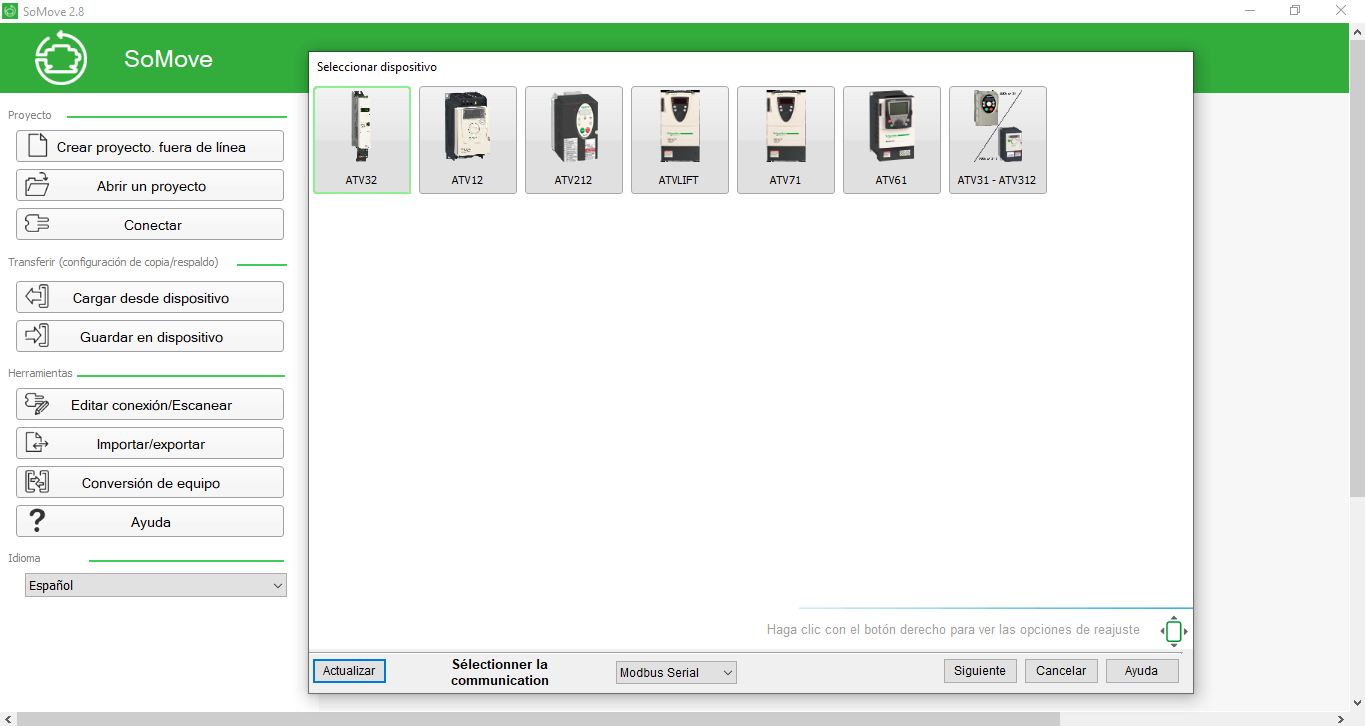
\includegraphics[scale=0.25]{somove1.png}
	\captionof{figure}{Elección de Altivar 312}
	\label{fig:so1}
\end{figure}
\begin{figure}[h]
	\centering
	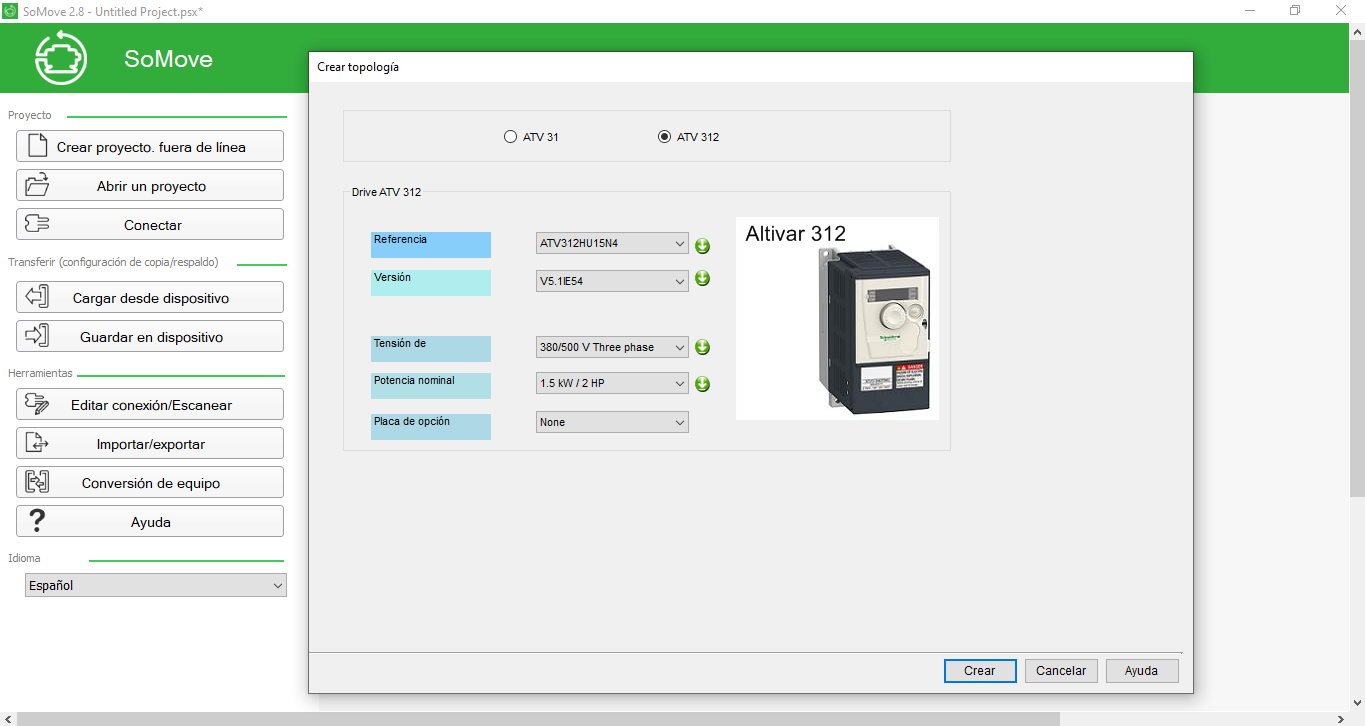
\includegraphics[scale=0.25]{somove2.png}
	\captionof{figure}{Parámetros del variador}
	\label{fig:so2}
	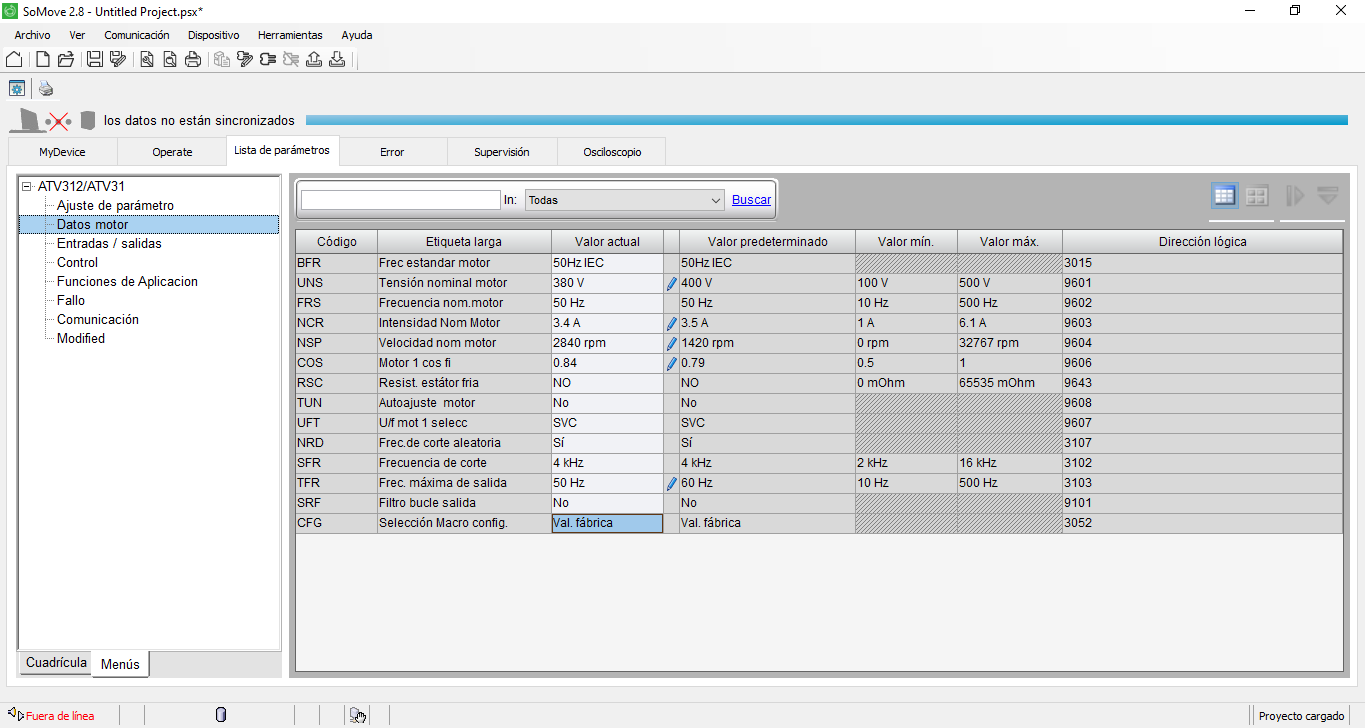
\includegraphics[scale=0.25]{somove4.png}
	\captionof{figure}{Configuración de los parámetros del motor}
	\label{fig:so4}
\end{figure}

Para realizar esta configuración se realizó la comunicación de la PC con el variador a través de \textbf{Modbus} (Figura\ref{fig:pcvar}).  
\begin{figure}[h]
	\centering
	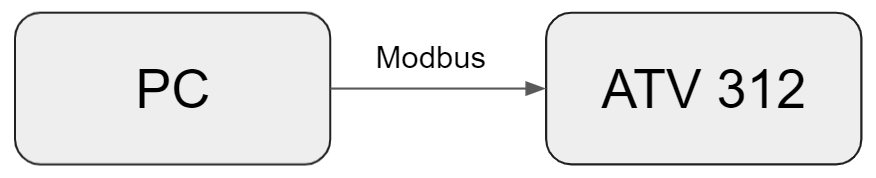
\includegraphics[scale=0.25]{pc_var.png}
	\captionof{figure}{Diegrama comunicación PC- Variador}
	\label{fig:pcvar}
\end{figure}

%Ver si CONFIGURACION DE COMUNICACION CANOPEN VA \hl{capaz que no va acá}
Ver si CONFIGURACION DE COMUNICACION CANOPEN VA \hl{va?}.

\subsubsection{Configuración de comunicación CANopen}

\begin{tcolorbox}[colback=blue!5!white,colframe=blue!75!black,title=CANopen]
	CANopen es un protocolo con aplicación industrial de bajo nivel para aplicaciones de automatización. Conecta dispositivos entre sí mediante mensajes entre pares. Basado en el estándar de comunicaciones físicas CAN. Se utiliza en redes de comunicación tipo esclavo, multimaestro. \hl{no me cierra esta definicion, buscar otra}
\end{tcolorbox}

\begin{tcolorbox}[colback=blue!5!white,colframe=blue!75!black,title=SDO]
	Objetos o mensajes de servicio utilizados para leer y escribir cualquiera de las entradas del diccionario de objetos de un dispositivo.
	Corresponden a mensajes CAN de baja prioridad.
\end{tcolorbox}

\begin{tcolorbox}[colback=blue!5!white,colframe=blue!75!black,title=PDO]
	Objetos o mensajes de proceso utilizados para el
	intercambio de datos de proceso, es decir, datos de tiempo real. Por este motivo,
	típicamente corresponden a mensajes CAN de alta prioridad.
\end{tcolorbox}


\paragraph{Registros a utilizar}
\hl{ir a ANEXO y poner la lista completa de direcciones}

\newpage

